\subsection{Análise anual}
Inicialmente, foram levantadas as quantidades de ligações registradas durante o ano e a quantidade total de falhas, assim como o percentual de falhas. No ano de 2021, que contou com 261 dias de trabalho, foram registradas 51.708 ligações, sendo que 4.227 destas demoraram mais de 60 segundos para serem atendidas, caracterizando falha do processo. O percentual destas falhas para o ano foi de 8,17\%, valor que atende as especificações de desempenho da empresa. No entanto, como este valor representa apenas uma média anual, devemos buscar compreender o problema da empresa ao avaliar o comportamento das variáveis relevantes do processo ao longo do ano.

\subsubsection{Quantidade de chamados por dia}
A Figura \ref*{fig: chamados-tempo} apresenta a quantidade de chamadas recebidas por dia ao longo do ano. É possível perceber uma relação de dependência entre a quantidade de ligações recebidas e os dias do ano, visto que o número de chamadas cresce ao longo do ano. Esse comportamento pode ser responsável pelo aumento do percentual de falhas em meses próximos ao fim do ano. Posteriormente, será descrito um estudo de regressão para estes dados.

\begin{figure}[h]
    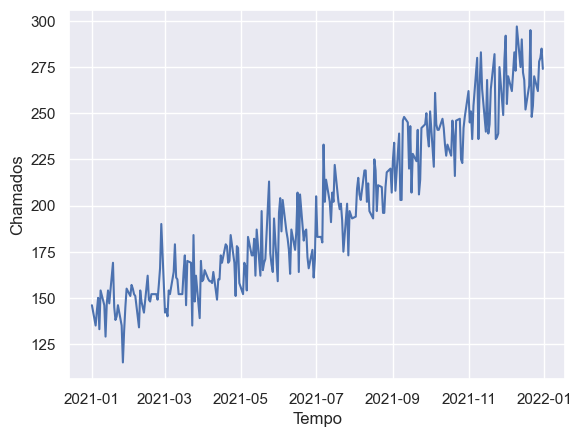
\includegraphics{analise-de-dados/anual/chamados.png}
    \caption{Quantidade de chamadas recebidas ao longo do tempo}
    \label{fig: chamados-tempo}
\end{figure}

\subsubsection{Análise e descrição dos tempos de espera e serviço}
Como os tempos de espera (\textit{wait length}) e serviço (\textit{service length}) já estão calculados, podemos analisar seu comportamento.

\begin{table}
\centering
    \begin{tabular}{lr}
        % \begin{center}
            \toprule
            {} &  Tempo de espera \\
            \midrule
            count &   51708.000  \\
            mean  &      17.035  \\
            std   &      64.061  \\
            min   &       0.000  \\
            25\%   &       0.000  \\
            50\%   &       0.000  \\
            75\%   &       0.000  \\
            max   &     983.000  \\
        % \end{center}
        \bottomrule
        % \label{tab: describe-wait}
    \end{tabular}
\caption{Estatística descritiva dos tempos de espera}
\label{tab: descricao-espera}
\end{table}

Teste
